Initially, I thought that to modify project to take into account a size of the release (amount of commits) will be pretty straightforward task. It actually was straightforward, but as always I've encountered several unexpected problems on the way. 

I intended to extend my previously used method from section \ref{ssec:gitReleaseDatesMining} which uses Git Api tags endpoint to get the release dates. Unfortunately I wasn't able to find number of commits in the returned objects. JSON object returned from API has following structure:

\begin{lstlisting}
  {
    "url": X,
    "assets_url": X,
    "upload_url": X,
    "html_url": X,
    "id": X,
    "tag_name": X,
    "target_commitish":X,
    "name": X,
    "draft": X,
    "author":{},
    "prerelease": X,
    "created_at": X,
    "published_at": X,
    "assets":[],
    "tarball_url": X,
    "zipball_url":X, 
    }
\end{lstlisting}

I've done some extra searching but didn't want to spend extra time so I've decided to go the way I knew will work. Instead of using Api to get the commit counts, I've crawled Github UI page of each release and extracted information directly from page source code. Each release details page provides information how many commits behind the current HEAD the commit is. The difference in this number between two following releases represents count of new commits for a release. Results of simple tabular substraction with spreadsheet formula needed to be manually corrected because projects often release several branches parallel and therefore substraction from the previous release was not always the correct one.

Eventually, I got correct number of commits for every release and could execute the same cross-correlation analysis described in the previous chapter, but this time instead of releases count, I've explored relationship between sentiment and commits count. One possible flaw in the commit count data are the pre-releases. I treated them as normal releases because they do offer new features but those very same commits are then counted in the official relaeses later on.

After getting the data ready I performed a stationarity test for commit counts. Sentiment values ar the same as before with count of releases. Results can be seen in table \ref{table:stationarity_table_commits} 

\begin{table}[H]
\centering
\begin{tabular}{ |p{3cm}||p{3cm}|p{3cm}|  }
 \hline
 \multicolumn{3}{|c|}{Stationarity test of web frameworks commit counts} \\
 \hline
 Framework & Dickey-Fuller & p-value\\
 \hline
 NodeJS   & -7.0239    &0.01\\ \hline
 AngularJS &   -2.547  & 0.3531\\ \hline
 EmberJS & -3.2764 & 0.0831\\ \hline
 VueJS    &-2.9748 & 0.1886\\ \hline
 CakePHP&   -3.655  & 0.03283\\ \hline
 Laravel& -2.919  & 0.2084\\ \hline
 Symfony& -4.8461  & 0.01\\ \hline
\end{tabular}
\caption{Stationarity test of commit counts}
\label{table:stationarity_table_commits}
\end{table}

I see that there are again several data series (AngularJS, EmberJS, VueJS, Laravel + NodeJS because of unstationarity of sentiment data) which are not stationary so exactly as before with release counts, I had to transform the data. After that, Pearson's cross correlation was calculated. Results for all 7 OSS projects can be seen in Figure \ref{fig:highestCorrelationsPlot}

\begin{figure}[H]%
    \centering
	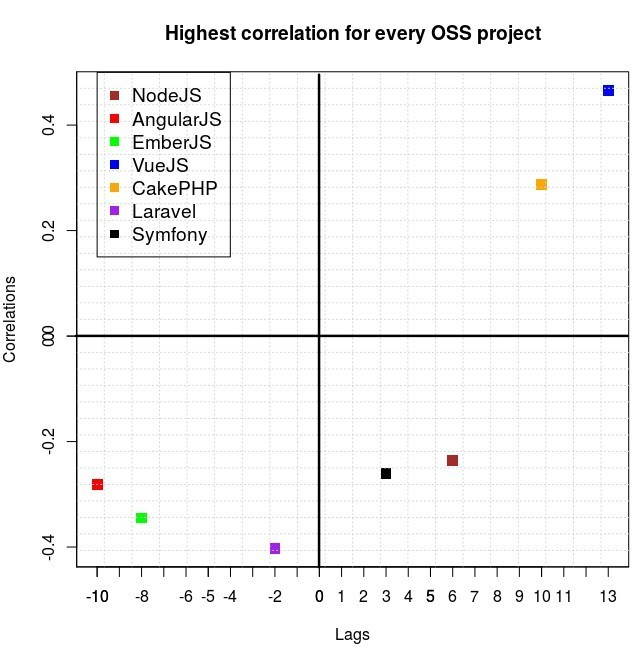
\includegraphics[width=8cm]{highestCorrelationsPlot.jpg}
    \caption{Highest correlations for every OSS project}%
    \label{fig:highestCorrelationsPlot}%
\end{figure}

If I would skip the step of making the data stationary, results would again look completely different \ref{fig:highestCorrelationsPlot_nonStat}.

\begin{figure}[H]%
    \centering
	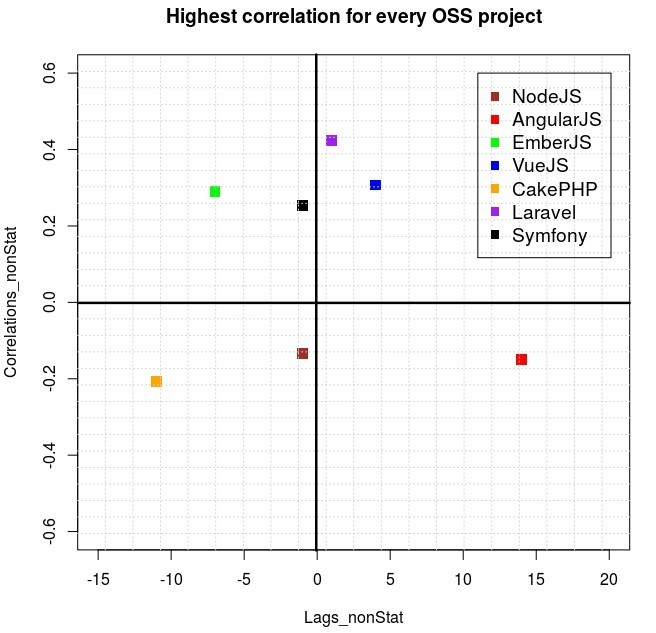
\includegraphics[width=8cm]{highestCorrelationsPlot_nonStat.jpg}
    \caption{Highest correlations for every OSS project (non-stationary)}%
    \label{fig:highestCorrelationsPlot_nonStat}%
\end{figure}